O Modelo de Domínio é construído para ilustrar os conceitos e relações entre estes, apresentando assim um modelo conceptual do problema em questão e nele podem ser visualizadas as entidades que participam na aplicação, assim como os papéis e atributos que desempenham. Nesse sentido, consideramos que este se trata de um modelo fulcral pois serve como um ponto de partida para toda a modelação.

\begin{figure}[H]
\centering
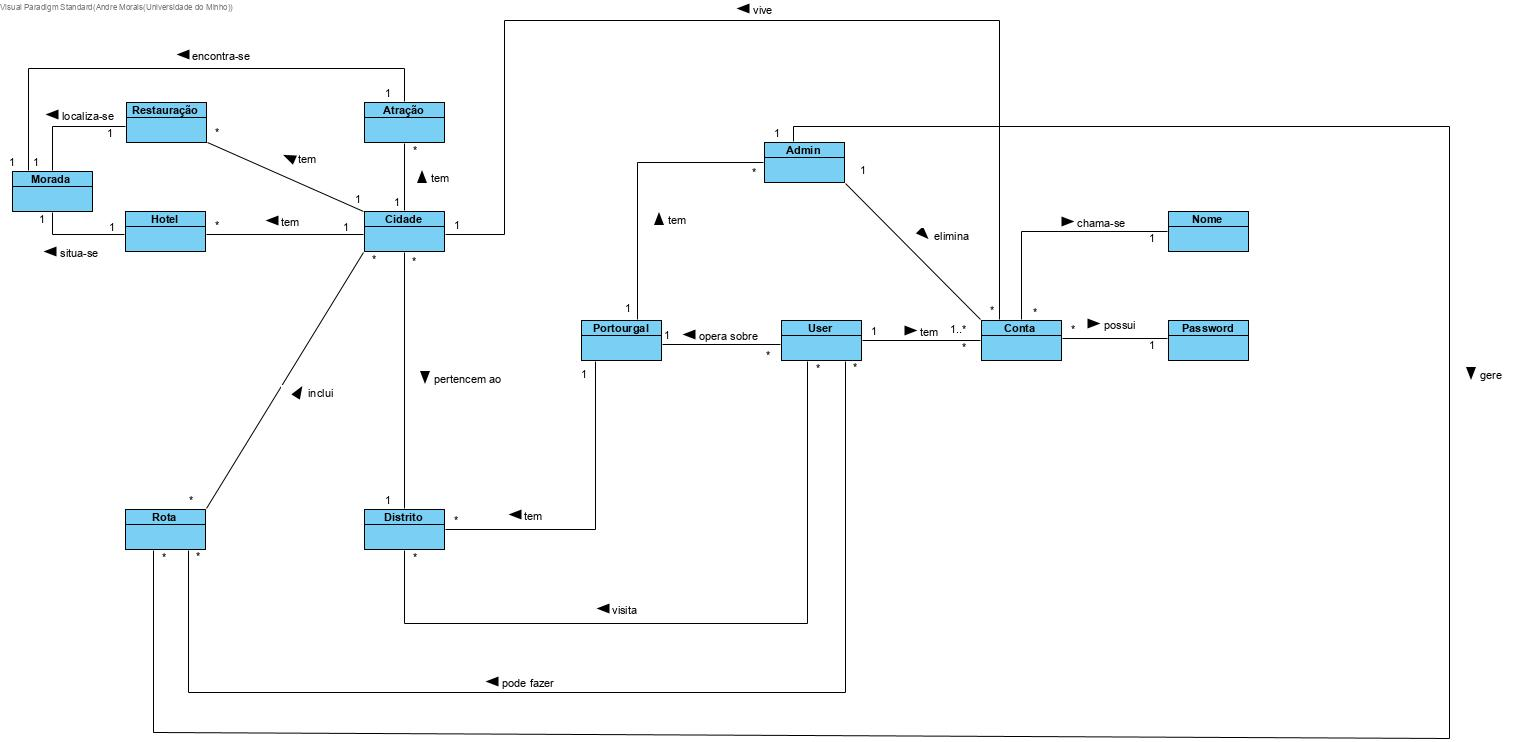
\includegraphics[width=0.9\linewidth]{images/modelodominio.jpg}
\caption{Modelo de Domínio}
\label{fig:mdominio}
\end{figure}

Consequentemente esboçamos a nossa versão, onde consideramos que as principais entidades do nosso sistema seriam: PORTOURGAL, User, Admin, Conta, Password, Nome, Distrito, Rota, Cidade, Atração, Morada, Restauração, Hotel.

Começando pelo PORTOURGAL a peça fundamental deste modelo, pois representa o “nome” da aplicação desenvolvida, que contêm Admins responsáveis pela aplicação, e para além disso é representada pelos Distritos. Os Users representam todos os utilizadores que vão operar/usar a aplicação, e estes terão uma Conta associada a cada um, com um Nome, Password e uma Cidade. Os Users operam sobre a PORTOURGAL de modo a visitar Cidades ou percorrer Rotas. As Rotas são identificadas por um conjunto de Cidades. Cada Cidade é identificada por Atrações, Restauração e Hotéis.